\IEEEraisesectionheading{\section{Introduction}\label{sec:intro}}
The ubiquity of location-acquisition devices leads to an explosive growth of movement data (i.e., trajectories), e.g., for vehicles, shared bikes and pedestrians. Visualizing these large-scale trajectory data is crucial for many smart city applications~\cite{wang2014visual,tang2017efficient,zheng2011learning} and location-based services~\cite{liu2016smartadp, zheng2010collaborative}. Among various visualization methods, line-based trajectory visualization, which connects the locations of a moving object by polylines, is widely adopted for spatial-temporal data analytics~\cite{chen2015survey,visualanalysis,bigchanvis}. To support interactive exploration on trajectory data, it is crucial to conduct  line-based trajectory visualization for an arbitrary target region with high quality and low latency.






%VLDB
%Nowadays, the ubiquity of location-acquisition devices leads to an explosive growth of the volume of movement data (i.e., trajectories), e.g., for vehicles, shared bikes and pedestrians. Visualizing these large-scale trajectory data is crucial for many smart city applications~\cite{wang2014visual,tang2017efficient,zheng2011learning} and location-based services~\cite{liu2016smartadp, zheng2010collaborative}. Among various visualization methods, line-based trajectory visualization, which connects the locations of a moving object by polylines, is widely adopted for spatial-temporal data analytics~\cite{chen2015survey,visualanalysis,bigchanvis}. However, large-scale line-based trajectory visualization suffers from two problems--(i) \textit{scalability} and (ii) \textit{visual clutter}, which we elaborate as follows.

%\textit{visual clutter}~\cite{kwon2017sampling}.




\stitle{Long visualization time for large-scale datasets} To visualize the trajectories in a target region $\query$, a natural solution is to find the trajectories in it and visualize all these trajectories ($\full$ for short). However, $\full$ may suffer from a long visualization time as the trajectory datasets can be extremely large. For example, Shenzhen has 24,237 taxis which collectively generate more than 7.72 million GPS locations each day~\cite{sz}. In addition, our profiling results in Table~\ref{tab:gpu}\footnote{Mapping is the time to map the GPS points to the screen points, and rendering is the time to render the screen points. The settings of this measurement can be found in Section~\ref{sec:exp}.} show that it takes 16.154 seconds to visualize the 1,000,000 taxi trajectories in the \pt{} dataset. As visualization time scales almost linearly with the number of trajectories (see Table~\ref{tab:gpu}), $\full$ could take a long time if there are many trajectories in the target region. However, interactive visual exploration typically requires the visualization to be generated in less than 1 second~\cite{shneiderman1984response}. Another problem of applying $\full$ on large-scale datasets is~\textit{visual clutter}~\cite{kwon2017sampling}, where there are too many points in the visualization such that it is difficult for human users to gain insights. We provide an example Figure~\ref{fig:overview}(A) for the \pt{} dataset, for which it is almost impossible to recognize the road networks in the dense region at the center.

\begin{table}
	\centering
	\small
	\caption{Visualization time on the \pt{} dataset (in seconds)}
    \trim
	\begin{tabular}{|c|c|c|c|c|} \hline
		No. of  & No. of & Mapping & Rendering & Total \\
         trajectories &  GPS points & time & time & time \\ \hline
		1,000& 31,300 & 0.027 & 0.003 & 0.03 \\ \hline
		10,000& 31,6531 & 0.169 & 0.005 & 0.174\\ \hline
		100,000& 316,7120 & 1.701 & 0.057 & 1.758 \\ \hline
		1,000,000& 31,646,379 & 15.562 & 0.592 & 16.154 \\ \hline
	\end{tabular}	\label{tab:gpu}
    \trim \trim 
\end{table}


%\stitle{Visual clutter} It is a common problem for large-scale data visualization, which we illustrate with an example in Figure~\ref{fig:overview}(A). Because of visual clutter, it is almost impossible to recognize the road network in the embedded figure of Figure~\ref{fig:overview}(A), making it difficult for human-users to gain insights from the visualization. Hence, we want the trajectory visualization to be visual-clutter-free for good user experience.

%VLDB
%\stitle{Scalability}
%Trajectory datasets can be extremely large and thus take a long time to render for visualization. For example, Shenzhen has 24,237 taxis which collectively generate more than 82.8 million GPS locations each day~\cite{sz}. Our benchmark on the \pt{} taxi trajectory dataset shows that it takes 13.95 seconds to render 1 million real-world trajectories using an NVIDIA GeForce GTX 1080 GPU with 8GB video memory. The long delay caused by large dataset cardinality makes interactive visual exploration difficult. Thus, we want visualization to scale to very large datasets while maintaining a short delay.


%In New York, {there are} over 13,000 taxis carrying over 1 million passengers and making 500,000 trips on an average day~\cite{ferreira2013visual}.

%Rendering refers to the use of the hardware device (e.g., GPU) in the generation of visualizations.

%However, the rendering capability of modern commodity GPUs is limited.
%We did a benchmark experiment to evaluate the rendering capability of NVIDIA GeForce GTX 1080 with 8GB video memory.
%It needs 13.95 seconds to render 1 million real-world trajectories in \pt{}. % with 32.66 millions GPS points.
%Obviously, it cannot support interactive visual exploration in large-scale trajectory dataset.
%Thus, how to support scalable visualization is the first challenge in large trajectory data visualization problem.



%It is almost impossible to
%
%It is a common issue in big data visualization~\cite{clutter}.
%Figure~\ref{fig:teaser}(A) is the visualization result of the full \pt{} taxi trajectory dataset.
%Intuitively, the region shown in the embedded figure of A suffers visual clutter issue seriously,
%i.e., the road network almost cannot be recognized in it,
%which hinders the abilities of human-users to explore the dataset and identify the underlying data insights.
%Hence, the second challenge in large trajectory data visualization problem is how to address visual clutter issue.



%To overcome the above challenges, several visualization approaches have been proposed in the literature.
%Unfortunately, none of them could address these three challenges simultaneously and perfectly.
%In particular, the spatial aggregation based approaches~\cite{zeng2013visualizing,von2015mobilitygraphs} preprocess the massive movement data, and visualize the results after preprocessing.
%The aggregation based methods ignored the visual clutter in raw spatial data as they only visualize the aggregated/preprocessed results.
%In other words, their visualization results may lose the detail information in raw data.
%%These approaches alleviate the large data size and limited rendering ability issues in large-scale spatial data visualization.
%%Nevertheless, they ignored the visual clutter issue in raw spatial data as they only visualize the aggregated/preprocessed results.
%In recent years, many visualization research works are proposed to address visual clutter,
%e.g., edge bundling~\cite{zeng2019route, thony2015vector} and density map~\cite{lampe2011interactive, scheepens2011interactive}.
%However, these works neither focus on line-based trajectory visualization nor designed for large-scale trajectory dataset.

% \begin{figure*}[t]
% 	\centering
% 	\includegraphics[width=0.90\textwidth]{pictures/Teaser.pdf}
% 	\vspace{-2mm}
% 	\caption{A comparison of visualization results. (I) A is the visualization of the full \pt{} taxi trajectory dataset at zoom level 11.
%     At the same zoom level, B and C are produced by uniform random sampling,
%     while D, E, F are produced by our $\avats$ algorithm.
%     (II) G is the visualization of the full \pt{} dataset at zoom level 15, while H and I are the corresponding results of uniform random sampling and $\avats$, respectively.
%     (III) F and I are generated by $\avats$ with color encoding for representativeness to combat visual clutter.
%     Best viewed in color.}
% 	\label{fig:teaser}
% \trim \trim
% \end{figure*}

% \QM{Introduce the data to visualization time: database/file - memory - data transformation(GPS to screen position)- visualization}.

\begin{figure*}[t]
	\centering
	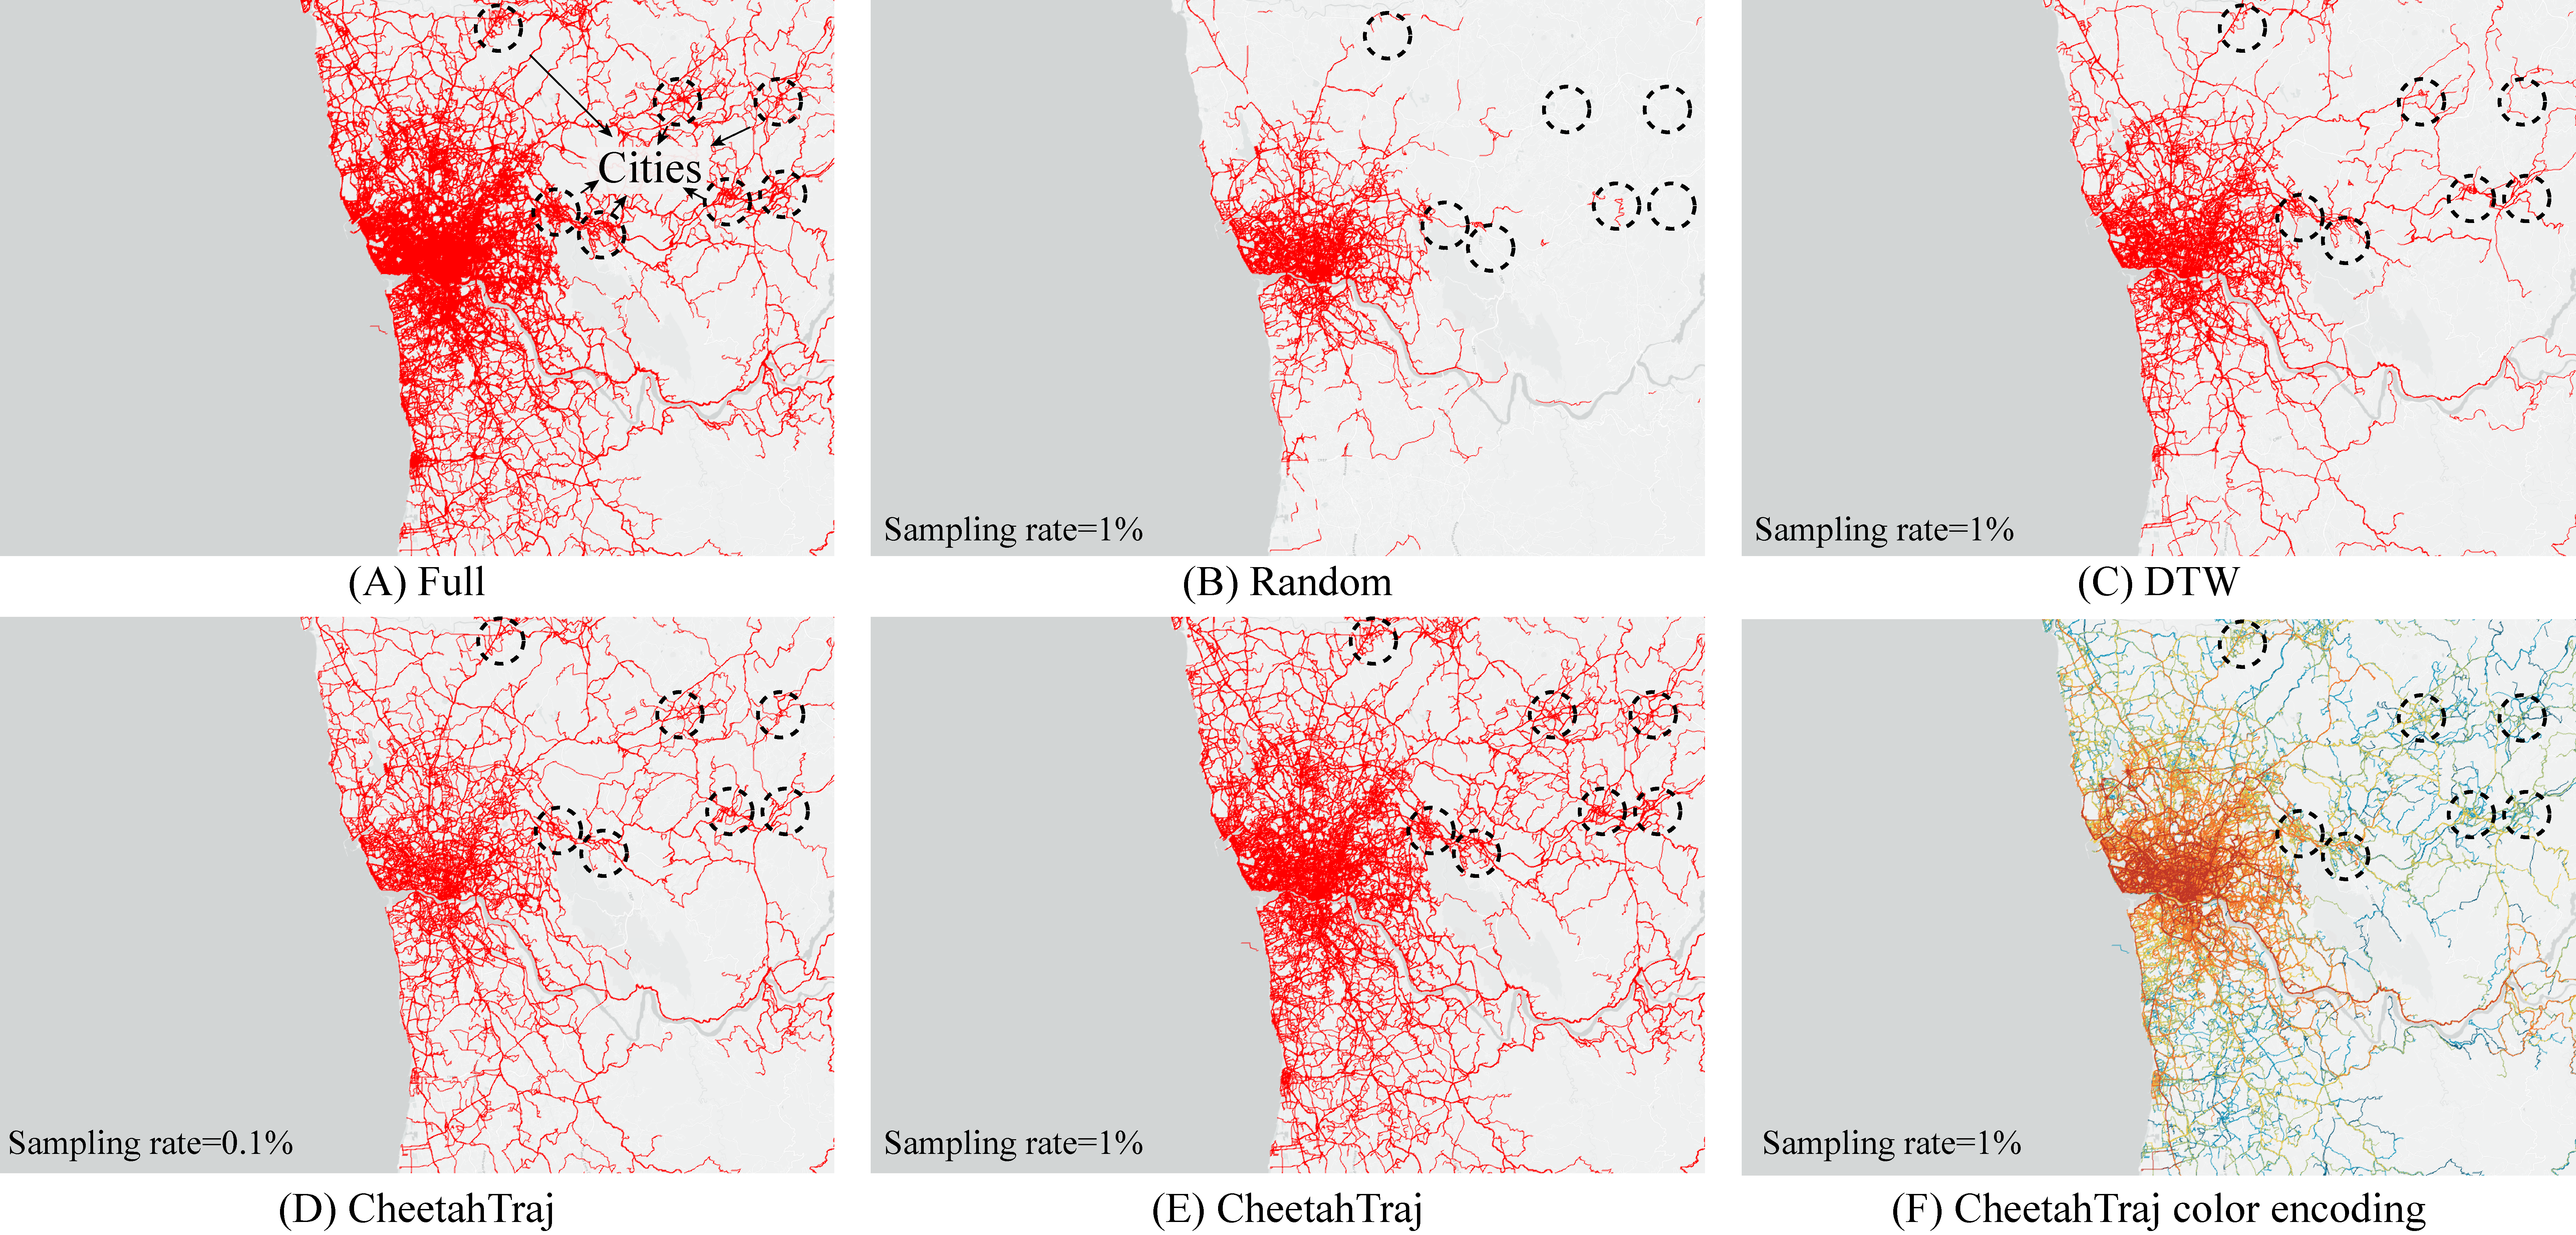
\includegraphics[width=0.98\textwidth]{pictures/case_study_icde/case_study_overview.pdf}
	\trim
	\caption{Effectiveness of $\avats$ at overview visualization in \pt{}.}
	\label{fig:overview}
	\trim \trim
\end{figure*}

\stitle{Ad-hoc sampling has poor visual quality} Sampling techniques are widely used to accelerate large-scale data analysis in both database and visualization communities~\cite{qin2020making,DBLP:conf/sigmod/DingHCC016,DBLP:journals/pvldb/KimBPIMR15,park2016visualization}. By selecting a subset of the trajectories in the target region for visualization, sampling can reduce both visualization time and visual clutter. One such example is ScalaR~\cite{battle2013dynamic}, which employs a reduction layer between the visualization layer and the data management layer. The reduction layer samples records \textit{uniformly at random} (denoted as $\rand$) when the query results are too large. However, $\rand$ has poor visual quality as its visualization could be significantly different from the ground-truth. We provide such an example in Figure~\ref{fig:overview}(B), where $\rand$ fails to include trajectories in the sparse areas of Figure~\ref{fig:overview}(A). Another natural idea is to sample trajectories with good diversity and we develop such a baseline using the famous Dynamic Time Warping (DTW) distance between trajectories~\cite{borcan2012improving}. As shown in Figure~\ref{fig:overview}(C), $\mathsf{DTW}$ provides better visualization than $\rand$ but there are still obvious differences between $\mathsf{DTW}$ and the ground-truth in Figure~\ref{fig:overview}(A). Without explicit visual quality guarantee, sampling trajectories in ad-hoc ways may produce visualizations with poor quality and mislead visual exploration.

% for trajectory
%
% basic idea
%
%for large-scale trajectory data visualization, generating visualizations that is significantly from the ground-truth. Take Figure~\ref{fig:overview}(B) for example, they are the visualization results generated by $\rand$ on the \pt{} taxi trajectory dataset with sampling rate  $1\%$. Obviously, it is very different from the visualization of the full \pt{} dataset in Figure~\ref{fig:overview}(A), since the random sampling method is easily ignore the data patterns in the spare areas.  Another basic idea of the data reduction is to iteratively remove the trajectories \QM{which have the least impact of the whole visualization}~\cite{borcan2012improving}. Thus impact of a trajectory can be evaluated by sum of the distance(DTW or Fréchet distance) to all other trajectories. As shown by Figure.~\ref{fig:overview}, the visualization generated $\baseline$ is much better than $Rand$ by preserve more trajectories in the sparse region, but the general structure is still missing because it cannot theoretically guarantee the visual quality. Moreover the pairwise distance calculation for large trajectory dataset is very time consuming, which always needs days of preprocessing for millions of trajectories.

%VLDB
%Sampling techniques are widely used for large-scale data analysis in both database and visualization communities~\cite{qin2020making,DBLP:conf/sigmod/DingHCC016,DBLP:journals/pvldb/KimBPIMR15,park2016visualization}. By sampling a subset of records from the raw large-scale dataset, it helps to reduce the rendering latency on graphics devices for visualization. One such example is ScalaR~\cite{battle2013dynamic}, which employs a reduction layer between the visualization layer and the data management layer. The reduction layer samples records \textit{uniformly at random} (denoted as $\rand$) when the query results are too large. However, $\rand$ does not work well for large-scale trajectory data visualization as it cannot provide fidelity guarantee. Take Figure~\ref{fig:teaser}(B) and (C) for example, they are the visualization results generated by $\rand$ on the \pt{} taxi trajectory dataset with sampling rate $0.1\%$ and $1\%$, respectively. Obviously, both of them are very different from the visualization of the full \pt{} dataset in Figure~\ref{fig:teaser}(A).


\stitle{The $\avats$ framework} We explore novel algorithm and efficient index jointly in the $\avats$ framework to provide visualizations with high quality and low latency. To conduct quality guaranteed sampling, we first propose a novel pixel-based \textit{visual quality function} to measure how similar an approximate visualization is to the ground-truth. We also show that it is NP-hard to select an optimal set of trajectories that maximize the visual quality function. Next, we devise a \textit{visual quality guaranteed sampling algorithm} named $\vats$, which provides theoretical visual quality guarantee for the sampled trajectories. Then, we \textit{tackle the visual clutter problem} by taking data distribution and human perception into consideration in an advance algorithm named $\vatss$. To avoid running the somehow complex $\vatss$ algorithm on-line for interactive visual exploration, we design an $\invQ$-tree index based on quad-tree. $\invQ$-tree allows to directly use the sampling results computed in an offline index building phase and provides quality guaranteed trajectory samples for an arbitrary target region.




%VLDB
%In this work, we set out to design efficient sampling algorithms that provides visual fidelity guarantee for line-based large-scale trajectory visualization. This goal leads to three research problems: (i) \emph{how to measure the visual fidelity of one visualization result?} (ii) \emph{how to devise an efficient sampling algorithm that provides  guaranteed visual fidelity?} (iii) \emph{how to tackle the visual clutter problem in large trajectory visualization?} To address these problems, we first propose a novel pixel-based \textit{visual fidelity loss function} to formally measure the difference between two visualizations. We then show that it is NP-hard to select a sized-$k$ sample of the trajectories to minimize the visual fidelity loss function. Next, we devise an \textit{efficient approximate algorithm }named $\vats$, which provides theoretical visual fidelity guarantee for the sampled results. Last, we \textit{explicitly tackle the visual clutter problem} by taking data distribution and human perception characteristics into consideration in an advance algorithm named $\avats$.

%In this work, we propose visual fidelity-guaranteed sampling approaches for the line-based trajectory visualization problem.
%The technical challenges of our proposal are
%(i) \emph{how to define visual fidelity of visualization result theoretically?}
%(ii) \emph{how to devise an efficient sampling algorithm which offers visual fidelity guarantee on the visualization result?}
%and (iii) \emph{how to overcome the visual clutter in large trajectory visualization?}
%Specifically, we first propose a novel pixel-based visual fidelity loss function between two visualization results formally.
%With the visual fidelity loss function, we then prove it is NP-hardness to select a sized-$k$ subset of trajectories which has the minimal visual fidelity loss.
%Next, we devise an approximate algorithm $\vats$ which returns a sized-$k$ subset of trajectories and offers theoretical visual fidelity guarantee on the returning result.
%Last, we address the visual clutter issue explicitly by taking data distribution and human perception capability into consideration in the advance approach $\avats$.



We conduct extensive case study, user study and quantitative performance evaluation to validate the visualization quality and efficiency of the $\avats$ framework. The case study shows that $\avats$ consistently provides high quality visualizations for both large target regions and small target regions. The user study with 35 participants confirms that $\avats$ effectively reduces visual clutter and produces visualizations that are plausible to human inspectors. The quantitative performance evaluation shows that $\avats$ provides good visual quality by sampling only a small number of trajectories. In addition,  $\avats$ produces high quality visualizations for arbitrary target regions in less than 1 second for all 3 experiment datasets and the visualation delay is below 0.1 second in most cases.


We illustrates the merits of our $\avats$ framework in Figure~\ref{fig:overview}. Figure~\ref{fig:overview}(D) and (E) are the visualizations produced by $\avats{}$ on the \pt{} dataset with sampling rate $0.1\%$ and $1\%$, respectively. Compared with uniform random sampling (i.e., $\rand$) and diversity based sampling (i.e., $\mathsf{DTW}$) in Figure~\ref{fig:overview}(B) and (C), Figure~\ref{fig:overview}(D) and (E) are obviously more similar to the full dataset visualization in Figure~\ref{fig:overview}(A).
Figure~\ref{fig:overview}(F) is produced by $\avats{}$ using the same parameters as Figure~\ref{fig:overview}(E) but the trajectories are colored according to their algorithm-generated representativeness (warmer color means more representative). Compared with Figure~\ref{fig:overview}(A), the main routes in the dense region can be identified much more easily, which shows that $\avats{}$ effectively reduces visual clutter. Last but not least, it takes $\avats{}$ only 0.116 seconds and 0.339 seconds to generate Figure~\ref{fig:overview}(D) and (E), respectively, while the full visualization in Figure~\ref{fig:overview}(A) takes 16.154 seconds.


% The advantage of our proposals over $\rand$ is also consistent across different zoom levels, e.g., Figure~\ref{fig:overview}(E) vs. Figure~\ref{fig:overview}(C) at level 11, and Figure~\ref{fig:overview}(I) vs. Figure~\ref{fig:overview}(H) at level 15. Figure~\ref{fig:overview}(F) is produced by our $\avats{}$ algorithm using the same parameters as Figure~\ref{fig:overview}(E) but the trajectories are colored according to their algorithm-generated representativeness (warmer color means more representative). Observe that the visual clutter problem in Figures~\ref{fig:overview}(A) and (E) are significantly alleviated in Figure~\ref{fig:overview}(F) with color encoding. This advantage is even more prominent when comparing Figure (I) with Figure (G) and (H).




%Figures~\ref{fig:teaser}(D) and (E) show the visualization results of our proposal $\avats{}$ on \pt{} taxi trajectory dataset with {the} sampling rate $0.1\%$ and $1\%$, respectively.
%Comparing with the corresponding visualization results of uniform random sampling method $\rand$ in Figure~\ref{fig:teaser}(B) and (C),
%the superiority of $\avats$ is obvious.
%% Obviously, the visualization fidelity of them are much better than the uniform random sampling visualization results with the same sampling rates, see Figure~\ref{fig:teaser}(B) and (C).
%Figures~\ref{fig:teaser}(F) is the returning result of our proposal, which colors the trajectories {according to the trajectory representativeness}.
%It has the same parameters of Figure~\ref{fig:teaser}(E).
%Visually, the visual clutter issue in Figures~\ref{fig:teaser}(A) and (E) are alleviated in Figure~\ref{fig:teaser}(F).
%In addition, our proposals are robustness with different zoom levels.
%%Figure~\ref{fig:teaser}(G), (H), and (I) depict the visualization results of the \pt{} dataset, the returning result of uniform random sampling $\rand$ and the returning result of $\avats$ with color encoding at zoom-level 15, for example, we can obtain them by zooming in the visualization result in Figure~\ref{fig:teaser}(A), (C), and (F), respectively.
%Consider the visualization results in Figures~\ref{fig:teaser}(G), (H), and (I) with zoom level 15.
%Intuitively, the visualization result of our proposal $\avats$ in Figure~\ref{fig:teaser}(F) outperforms the uniform random sampling $\rand$ in Figure~\ref{fig:teaser}(H) significantly.
%It even performs better than Figure~\ref{fig:teaser}(G), the visualized result of the \pt{} dataset, as it reduces visual clutter in Figure~\ref{fig:teaser}(G) by using color encoding scheme to capture the representativeness of different trajectories.

To sum up, our technical contributions in this paper include:
%\setlist{nolistsep}
%\begin{itemize}[noitemsep]
\squishlist
  \item We formulate the visual quality optimal trajectory sampling problem for large-scale trajectory data visualization, and prove that it is {NP-hard} (Section~\ref{sec:pro}).
  \item We devise an approximate algorithm $\vats$ for the visual quality guaranteed sampling problem. $\vats$ is further improved with $\vatss$ by considering data distribution and human perception (Section~\ref{sec:sol}).
  \item We propose the $\avats$ framework, which jointly uses the aforementioned algorithms and tailored index to achieve both quality and efficiency in large-scale trajectory data visualization (Section~\ref{sec:cheetahtraj}).

   %We conduct extensive experiments on real-world trajectory datasets to demonstrate the superiority of our proposals in Section~\ref{sec:exp}. In particular, nearly 200 real users are recruited to test the effectiveness of our methods on three practical applications.
\squishend
%\end{itemize}


This rest of the paper is organized as follows. Section~\ref{sec:rel} introduces related works on trajectory visualization and interactive visualization. The quality optimal trajectory sampling problem is formulated and analyzed in Section~\ref{sec:pro}. Section~\ref{sec:sol} presents our $\vats$ and $\vatss$ algorithm for quality guaranteed trajectory sampling. Section~\ref{sec:cheetahtraj} elaborates the $\avats$ framework. The experiment results are presented in Section~\ref{sec:exp}. Section~\ref{sec:con} draws the concluding remarks.


% in Section~\ref{sec:pro}

%Our proposal demonstrates their superiority over existing methods
%With the same sampling set size($1\%$), the proposed method generates a higher-fidelity visualization and .

%With the loss function, we analyze the hardness of the problem, and devise a visual quality guaranteed sampling algorithm for it.
%Figure~\ref{fig:compare} depicts an comparison among the ground truth,  uniform random sampling and our proposed method.
%With the same sampling set size($1\%$), the proposed method generates a higher-fidelity visualization and support the multi-resolution very well.
%At last, color encoding are applied to enhance the distribution of trajectories.

%


%\TB{Visualizing a large collection of trajectories are used frequently in map service or smart city applications.}
%The most popular and conventional method is the line-based visualization~\cite{chen2015survey}: connecting the passing points of movement objects by polylines.
%To handle the big dataset, many visualization products such as Spotfire~\footnote{\url{https://www.tibco.com/products/tibco-spotfire}}
%and Tableau~\footnote{\url{https://www.tableau.com/}} support advanced database management systems as a ``backend'' for the efficient data processing the query.
%The current visualization tools always don't scale well for the presentation of very large trajectory dataset due to the two challenges,
%visual clutter and limited rendering speed, which hinders the abilities of human-users for interactively exploring the dataset and identifying the movement patterns.
%In recent years, most of the visualization research works mainly try to address the visual clutter issue by proposing new techniques such as the
%spatial aggregation~\cite{zeng2013visualizing, von2015mobilitygraphs}, edge bundling~\cite{zeng2019route, thony2015vector} and density map~\cite{lampe2011interactive, scheepens2011interactive}.
%Instead, in this paper, we focus on the challenge of inefficient rendering in the large trajectory dataset by involving data sampling techniques.

%It is time consuming to generate very simple visualization when the data size become very large. Using Porto taxi data ~\footnote{\url{http://www.geolink.pt/ecmlpkdd2015-challenge/dataset.html}} as an example, Table~\ref{table:rendering_time} demonstrates the rendering time at each dataset size. \ZW{shall also mention which rendering toolkit is used here.} It shows that normal method takes more than 14 minutes (\ZW{seconds?}) to generate the graphics for 1 million trajectories, which is far beyond the human-acceptable response time for the interactive exploration~\cite{shneiderman1984response}.
%One work closely related to ours is ScalaR~\cite{battle2013dynamic}, which adds a reduction layer between visualization layer and data management layer. The reduction layer uses an uniform random sampling method to sample data once the query results are large enough, thus to reduce the amount of data to be visualized.
%Further more, Park et al. propose VAS~\cite{park2016visualization} which implements new sampling techniques to guarantee the visual quality.
%However, these sampling techniques are designed for the simple dataset, and have been approved effective in scatter plot or map plot.
%However, the trajectory sampling is more challenge due to the complexity of data form(e.g. varying lengths, lack of compact representation, difficulty in measuring the similarity) that makes traditional density-biased sampling techniques inappropriate.
%A naive solution to employ sampling idea for large-scale trajectory visualization problem is randomly selecting several trajectories from the data set then visualize it by graphics device.
%However, the visualization result may be not acceptable by the user because of the visual information loss in the sparse distributed regions.





%
%\begin{figure}[t]
%	\centering
%	\includegraphics[width=0.4\textwidth]{pictures/introduction/timesize.png}
%	\vspace{-5mm}
%	\caption{The latency time for generating line-based visualization at each datasize.}
%	\vspace{-5mm}
%	\label{fig:rendering_time}
%\end{figure}




%The major challenges to design visual quality guaranteed sampling method are:
%(I) how to define visual quality theoretically? (II) how to guarantee the quality of the sampling-based visualization result?
%\TB{In this work, we study how to reduce the rendering time and preserve the visual quality for the large-scale trajectory visualization.}
%We extend the motivation of visualization-aware sampling to trajectory dataset and propose a novel sampling strategy, \textbf{v}isualization \textbf{a}ware \textbf{t}rajectory \textbf{s}ampling(VATS), that produces high-visual-quality line-based trajectory visualization at different zooming resolutions.
%%\QM{In this paper, we first proposed the visual fidelity loss function which effectively evaluates the visual loss of the sampling method. Then we minimize the loss function by transforming this problem to an optimization problem. Several solutions for efficiently solving the optimization problem are discussed.}
%We first format visual quality by defining the loss function between the visualization results of the whole dataset and sampled dataset.
%With the loss function, we analyze the hardness of the problem, and devise a visual quality guaranteed sampling algorithm for it.
%Figure~\ref{fig:compare} depicts an comparison among the ground truth,  uniform random sampling and our proposed method.
%With the same sampling set size($1\%$), the proposed method generates a higher-fidelity visualization and support the multi-resolution very well.
%At last, color encoding are applied to enhance the distribution of trajectories.
%
%\begin{figure}[t]
%	\centering
%	\includegraphics[width=0.44\textwidth]{pictures/introduction/effectiveness.pdf}
%	\vspace{-3mm}
%	\caption{Trajectory sampling generated by uniform random sampling(A,C) and VQGTS(B,D) at same sampling rate. In both high-level(A,B) and low level(C,D) view, our approach preserved more detail information about the trajectories especially for the sparse regions.}
%	\vspace{-5mm}
%	\label{fig:compare}
%\end{figure}
%

%
% \Bo{we can keep it at technical report.}
%The remainder of this paper is organized as follows. Section~\ref{sec:rel} discusses the related work, and Section~\ref{sec:pro} formally formulates our problem and analyze its hardness. Section~\ref{sec:sol} presents our approximate solution for the problem along with the optimization techniques. The advanced solution for visual clutter is introduced in Section~\ref{sec:aa}. Section~\ref{sec:exp} elaborates the extensive experimental studies. Section~\ref{sec:con} concludes this paper and highlights possible future directions.


%Section~\ref{sec:pro} formulates our problem and analyze its hardness.
%Section~\ref{sec:sol} provides an approximate solution for it, together with a suite of optimization techniques.
%Section~\ref{sec:aa} proposes an advanced solution for our problem.
%Section~\ref{sec:exp} elaborates our extensive experimental studies and our findings in detail.
%Section~\ref{sec:con} concludes this work and highlights the promising future directions.

